\documentclass[11pt,a4paper]{article}
\XeTeXlinebreaklocale "zh"
\XeTeXlinebreakskip = 0pt plus 1pt minus 0.1pt
\usepackage[top=1in,bottom=1in,left=1.25in,right=1.25in]{geometry}
\usepackage{float}
\usepackage{fontspec}
\newfontfamily\zhfont[BoldFont=STHeiti]{STFangsong}
\newfontfamily\zhpunctfont{STFangsong}
\setmainfont{Times New Roman}
\usepackage{indentfirst}
\usepackage{zhspacing}
\zhspacing

% 代码展示
\usepackage{color}
\definecolor{bg}{rgb}{0.152941, 0.156863, 0.133333}
\usepackage{minted}
\usemintedstyle{monokai}
\setmonofont{DejaVuSansMono}

\usepackage{fancyvrb}  % 调整 Verbatim 中字体

% 调整 quotation 字体
\let\quotationOLD\quotation
\def\quotation{\quotationOLD\footnotesize}

\usepackage{pdfpages}  % 附上 pdf 版综合结果

\begin{document}

\title{作业 1}
\author{无36$\quad$李思涵$\quad$2013011187}
\maketitle


\section{投票器}

\subsection{电路结构}
\begin{figure}[H]
  \centering
    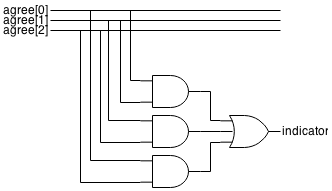
\includegraphics{../../homework1/1_voter/h1_p1}
  \caption{投票器}
\end{figure}

\subsection{代码}
\subsubsection{元件代码}
\inputminted[bgcolor=bg, linenos=true, fontsize=\footnotesize]{verilog}
{../../homework1/1_voter/voter.v}

\subsubsection{测试代码}
\inputminted[bgcolor=bg, linenos=true, fontsize=\footnotesize]{verilog}
{../../homework1/1_voter/voter_tb.v}

\subsection{仿真结果}
\VerbatimInput[fontsize=\scriptsize, numbers=left]{../../homework1/1_voter/result.txt}


\section{毕业判断器}

\subsection{电路结构}
\begin{figure}[H]
  \centering
    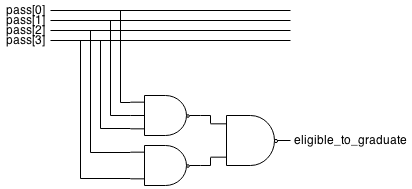
\includegraphics{../../homework1/2_graduate_judger/h1_p2}
  \caption{投票器}
\end{figure}

\subsection{代码}
\subsubsection{元件代码}
\inputminted[bgcolor=bg, linenos=true, fontsize=\footnotesize]{verilog}
{../../homework1/2_graduate_judger/graduate_judger.v}

\subsubsection{测试代码}
\inputminted[bgcolor=bg, linenos=true, fontsize=\footnotesize]{verilog}
{../../homework1/2_graduate_judger/graduate_judger_tb.v}

\subsection{仿真结果}
\VerbatimInput[fontsize=\scriptsize, numbers=left]{../../homework1/2_graduate_judger/result.txt}


\section{路灯控制器}

\subsection{电路结构}
\begin{figure}[H]
  \centering
    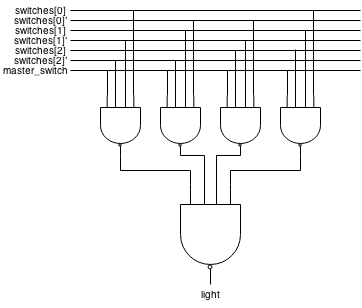
\includegraphics{../../homework1/3_street_light_controller/h1_p3}
  \caption{投票器}
\end{figure}

\subsection{代码}
\subsubsection{元件代码}
\inputminted[bgcolor=bg, linenos=true, fontsize=\footnotesize]{verilog}
{../../homework1/3_street_light_controller/street_light_controller.v}

\subsubsection{测试代码}
\inputminted[bgcolor=bg, linenos=true, fontsize=\footnotesize]{verilog}
{../../homework1/3_street_light_controller/street_light_controller_tb.v}

\subsection{仿真结果}
\VerbatimInput[fontsize=\scriptsize, numbers=left]{../../homework1/3_street_light_controller/result.txt}


\section{温度码-BCD码转换器}

\subsection{电路结构}
\begin{figure}[H]
  \centering
    
\includegraphics{../../homework1/4_thermometer_to_bcd/h1_p4}
  \caption{投票器}
\end{figure}

\subsection{代码}
\subsubsection{元件代码}
\inputminted[bgcolor=bg, linenos=true, fontsize=\footnotesize]{verilog}
{../../homework1/4_thermometer_to_bcd/thermometer_to_bcd.v}

\subsubsection{测试代码}
\inputminted[bgcolor=bg, linenos=true, fontsize=\footnotesize]{verilog}
{../../homework1/4_thermometer_to_bcd/thermometer_to_bcd_tb.v}

\subsection{仿真结果}
\VerbatimInput[fontsize=\scriptsize, numbers=left]{../../homework1/4_thermometer_to_bcd/result.txt}


\section{原码补码转换器}

\subsection{电路结构}
\begin{figure}[H]
  \centering
    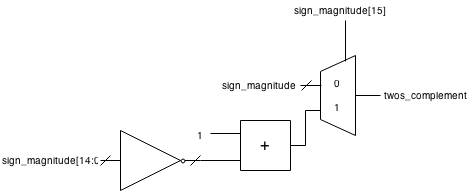
\includegraphics{../../homework1/5_sign_magnitude_to_twos_complement/h1_p5}
  \caption{投票器}
\end{figure}

\subsection{代码}
\subsubsection{元件代码}
\inputminted[bgcolor=bg, linenos=true, fontsize=\footnotesize]{verilog}
{../../homework1/5_sign_magnitude_to_twos_complement/sign_magnitude_to_twos_complement.v}

\subsubsection{测试代码}
\inputminted[bgcolor=bg, linenos=true, fontsize=\footnotesize]{verilog}
{../../homework1/5_sign_magnitude_to_twos_complement/sign_magnitude_to_twos_complement_tb.v}

\subsection{仿真结果}
\VerbatimInput[fontsize=\scriptsize, numbers=left]{../../homework1/5_sign_magnitude_to_twos_complement/result.txt}


\section{分频器}

\subsection{电路结构}
\begin{figure}[H]
  \centering
    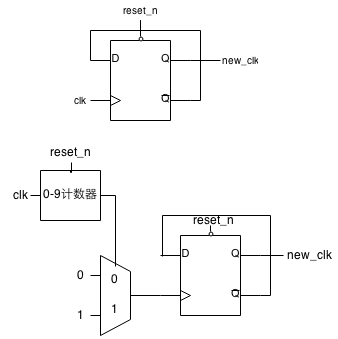
\includegraphics{../../homework1/6_watchmaker/h1_p6}
  \caption{投票器}
\end{figure}

\subsection{代码}
\subsubsection{元件代码}
\inputminted[bgcolor=bg, linenos=true, fontsize=\footnotesize]{verilog}
{../../homework1/6_watchmaker/watchmaker.v}

\subsubsection{测试代码}
\inputminted[bgcolor=bg, linenos=true, fontsize=\footnotesize]{verilog}
{../../homework1/6_watchmaker/watchmaker_tb.v}

\subsection{仿真结果}
\VerbatimInput[fontsize=\scriptsize, numbers=left]{../../homework1/6_watchmaker/result.txt}


\section{序列检测器}

\subsection{电路结构}
\begin{figure}[H]
  \centering
    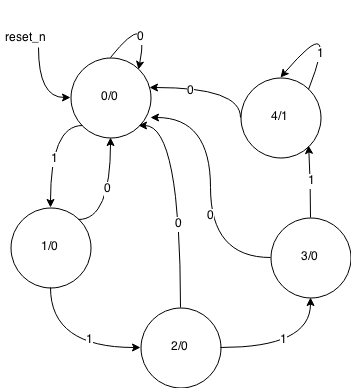
\includegraphics{../../homework1/7_seq_detector/h1_p7}
  \caption{投票器}
\end{figure}

\subsection{代码}
\subsubsection{元件代码}
\inputminted[bgcolor=bg, linenos=true, fontsize=\footnotesize]{verilog}
{../../homework1/7_seq_detector/sequence_detector_fsm.v}

\subsubsection{测试代码}
\inputminted[bgcolor=bg, linenos=true, fontsize=\footnotesize]{verilog}
{../../homework1/7_seq_detector/sequence_detector_fsm_tb.v}

\subsection{仿真结果}
\VerbatimInput[fontsize=\scriptsize, numbers=left]{../../homework1/7_seq_detector/result.txt}


\section{序列生成器}

\subsection{电路结构}
\begin{figure}[H]
  \centering
    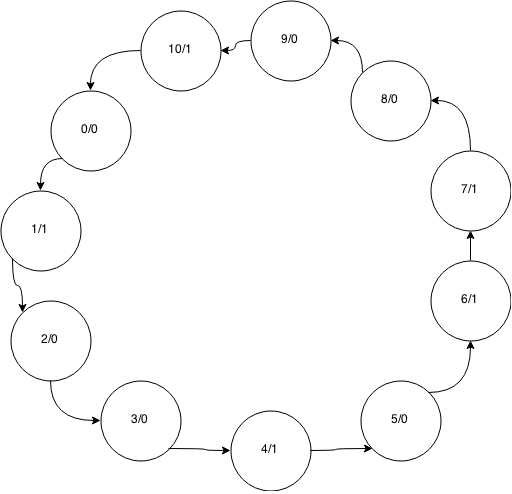
\includegraphics{../../homework1/8_seq_generator/h1_p8}
  \caption{投票器}
\end{figure}

\subsection{代码}
\subsubsection{元件代码}
\inputminted[bgcolor=bg, linenos=true, fontsize=\footnotesize]{verilog}
{../../homework1/8_seq_generator/seq_generator.v}

\subsubsection{测试代码}
\inputminted[bgcolor=bg, linenos=true, fontsize=\footnotesize]{verilog}
{../../homework1/8_seq_generator/seq_generator_tb.v}

\subsection{仿真结果}
\VerbatimInput[fontsize=\scriptsize, numbers=left]{../../homework1/8_seq_generator/result.txt}

\end{document}

